\documentclass{book}
\usepackage[left=2cm, right=2cm, top=2cm, bottom=2cm]{geometry}

\usepackage[spanish]{babel}
\usepackage[utf8]{inputenc}

\usepackage{pdfpages}
\usepackage[pdftex,pdfpagelabels=true,bookmarks=true]{hyperref} % Para enlaces y metadatos
\usepackage{bookmark}
\usepackage{fontawesome5}
\usepackage{fancyhdr}
\usepackage{titletoc}

\hypersetup{
    colorlinks=true,
    linkcolor=black,  % Color de los enlaces internos (por ejemplo, dentro de la tabla de contenidos)
    urlcolor=magenta,   % Color de los enlaces a URLs
    %%citecolor=green,
    pdfauthor={Moisés Serrano Samudio},
    pdftitle={Villancicos Populares},
    pdfsubject={Partituras},
    pdfkeywords={violín, trío, villancicos, navidad}
}

\title{Villancicos Populares}
\author{Moisés Serrano Samudio}
\date{\today}

\begin{document}

\newcommand{\CoverName}{Portada}%
\pagestyle{empty}%
\renewcommand{\thepage}{\CoverName}
\includepdf[pages=-]{../extend/0-portada.pdf}

\renewcommand{\CoverName}{Portadilla}%
\pagestyle{empty}%
\renewcommand{\thepage}{\CoverName}
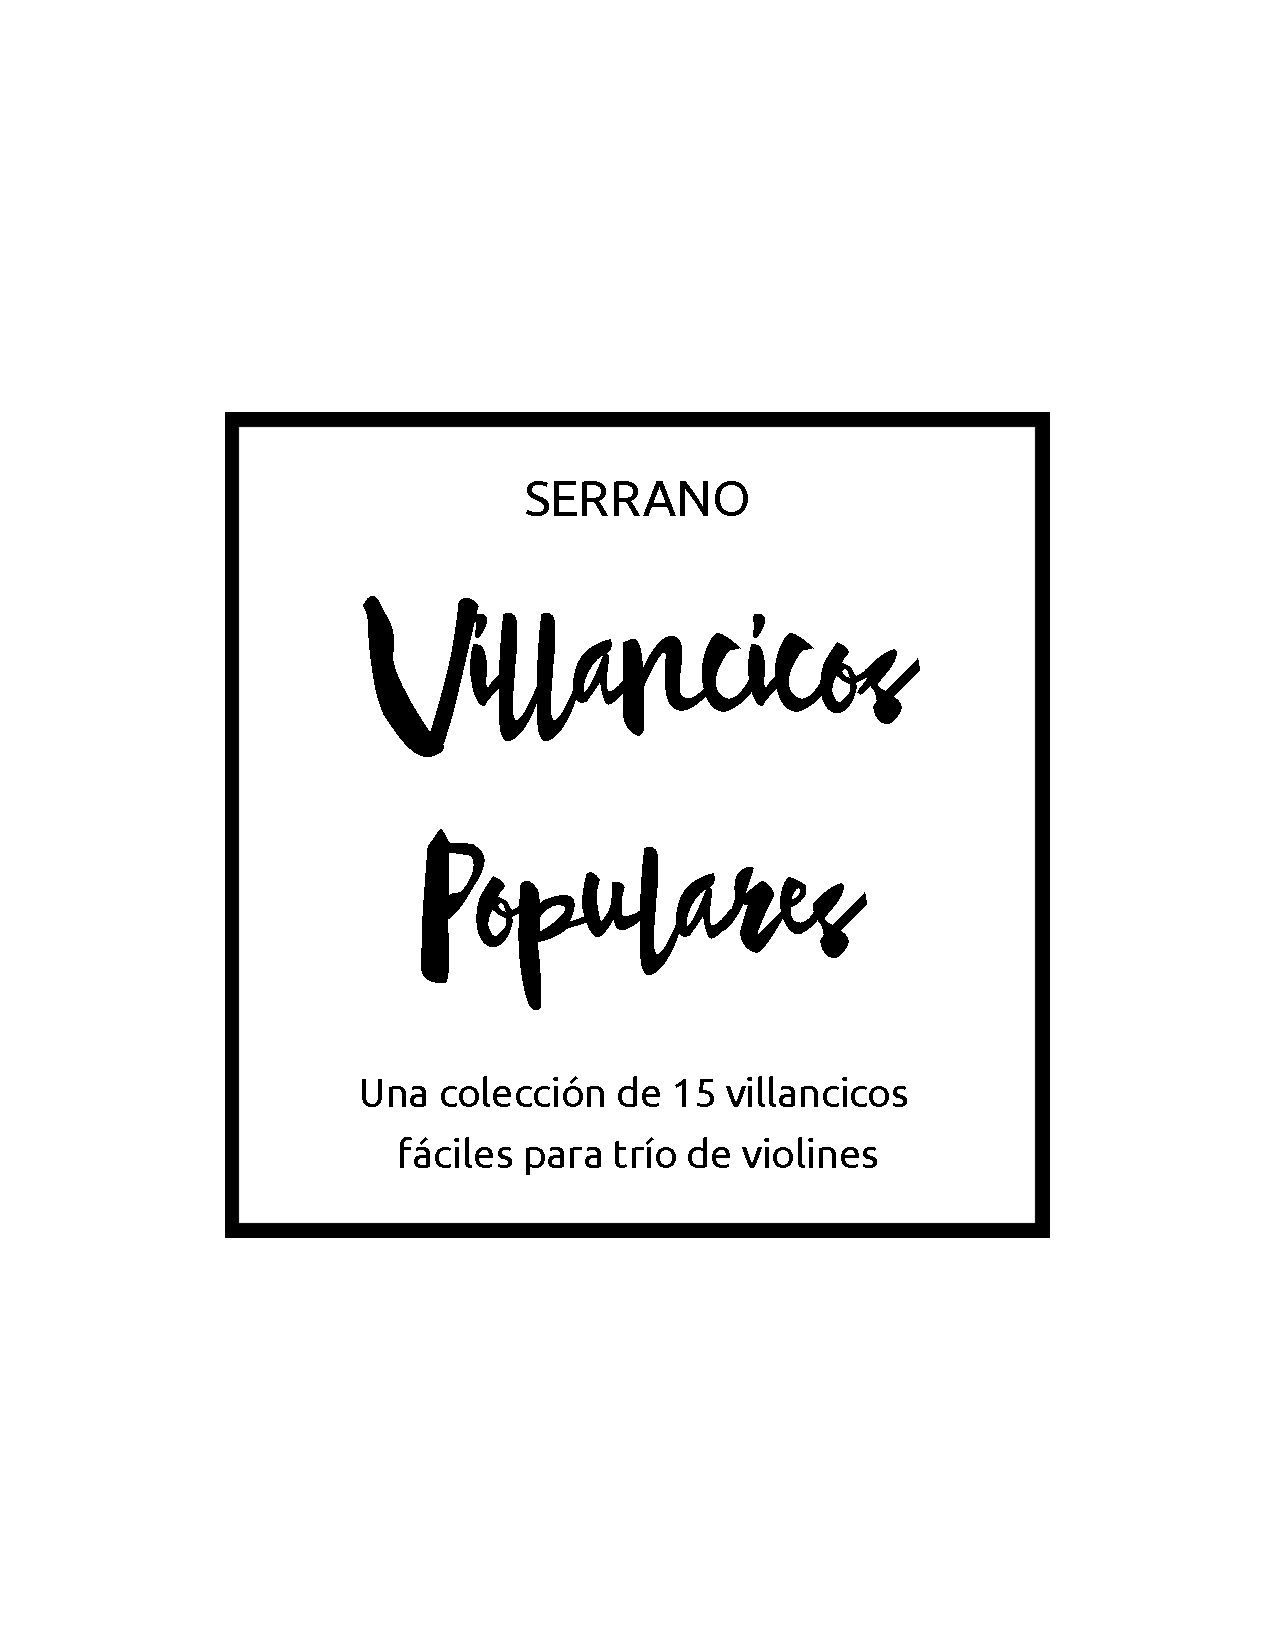
\includepdf[pages=-]{../extend/1-portadilla.pdf}

\renewcommand{\CoverName}{Licencia}%
\pagestyle{empty}%
\renewcommand{\thepage}{\CoverName}
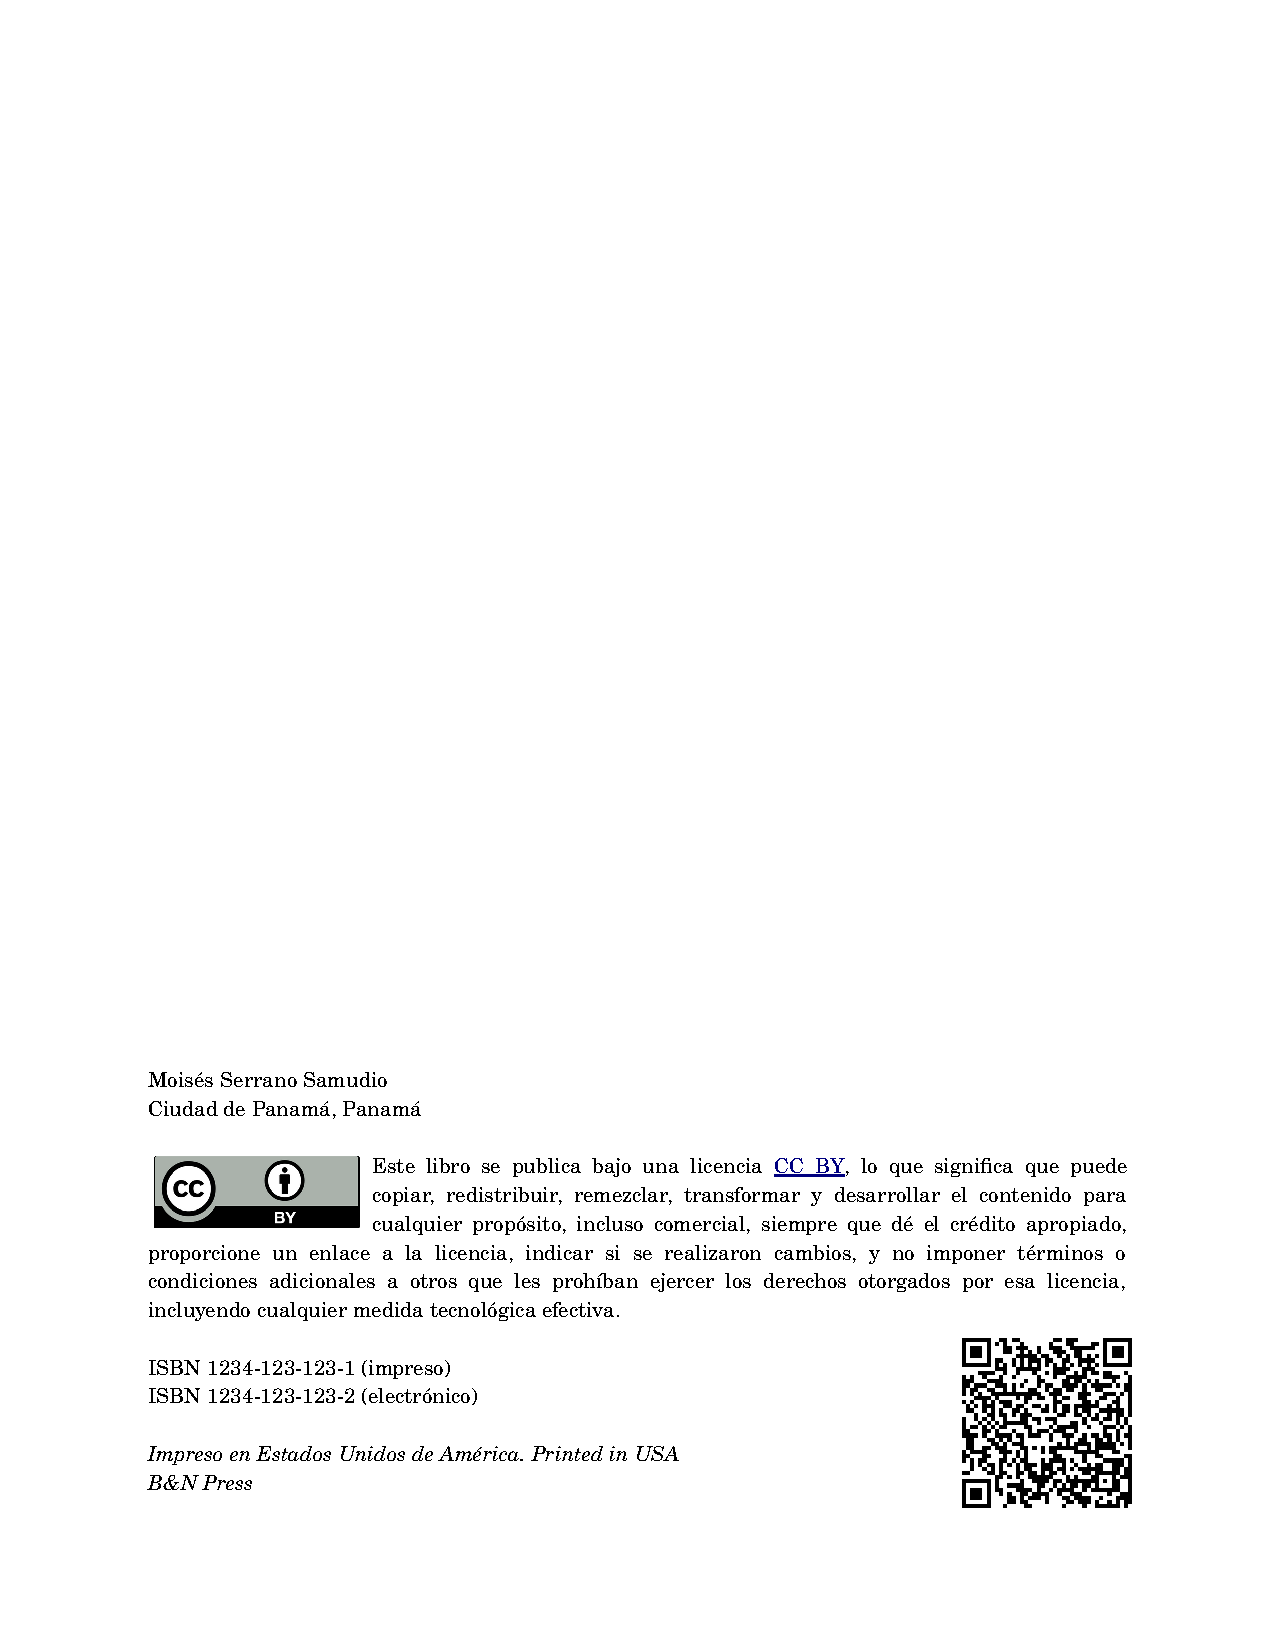
\includepdf[pages=-]{../extend/2-licencia.pdf}

\pagenumbering{roman}

%% Tabla de contenidos
\renewcommand{\contentsname}{Índice} %% Índice de partituras
% Establecer los márgenes de la página de índice
\newgeometry{left=5cm, right=5cm, top=2cm, bottom=2cm}
\pdfbookmark{\contentsname}{Partituras}
\tableofcontents
\restoregeometry 
% Volver a ajustar los márgenes después de índice a los originales


\includepdf[pages=-]{../extend/blank.pdf}
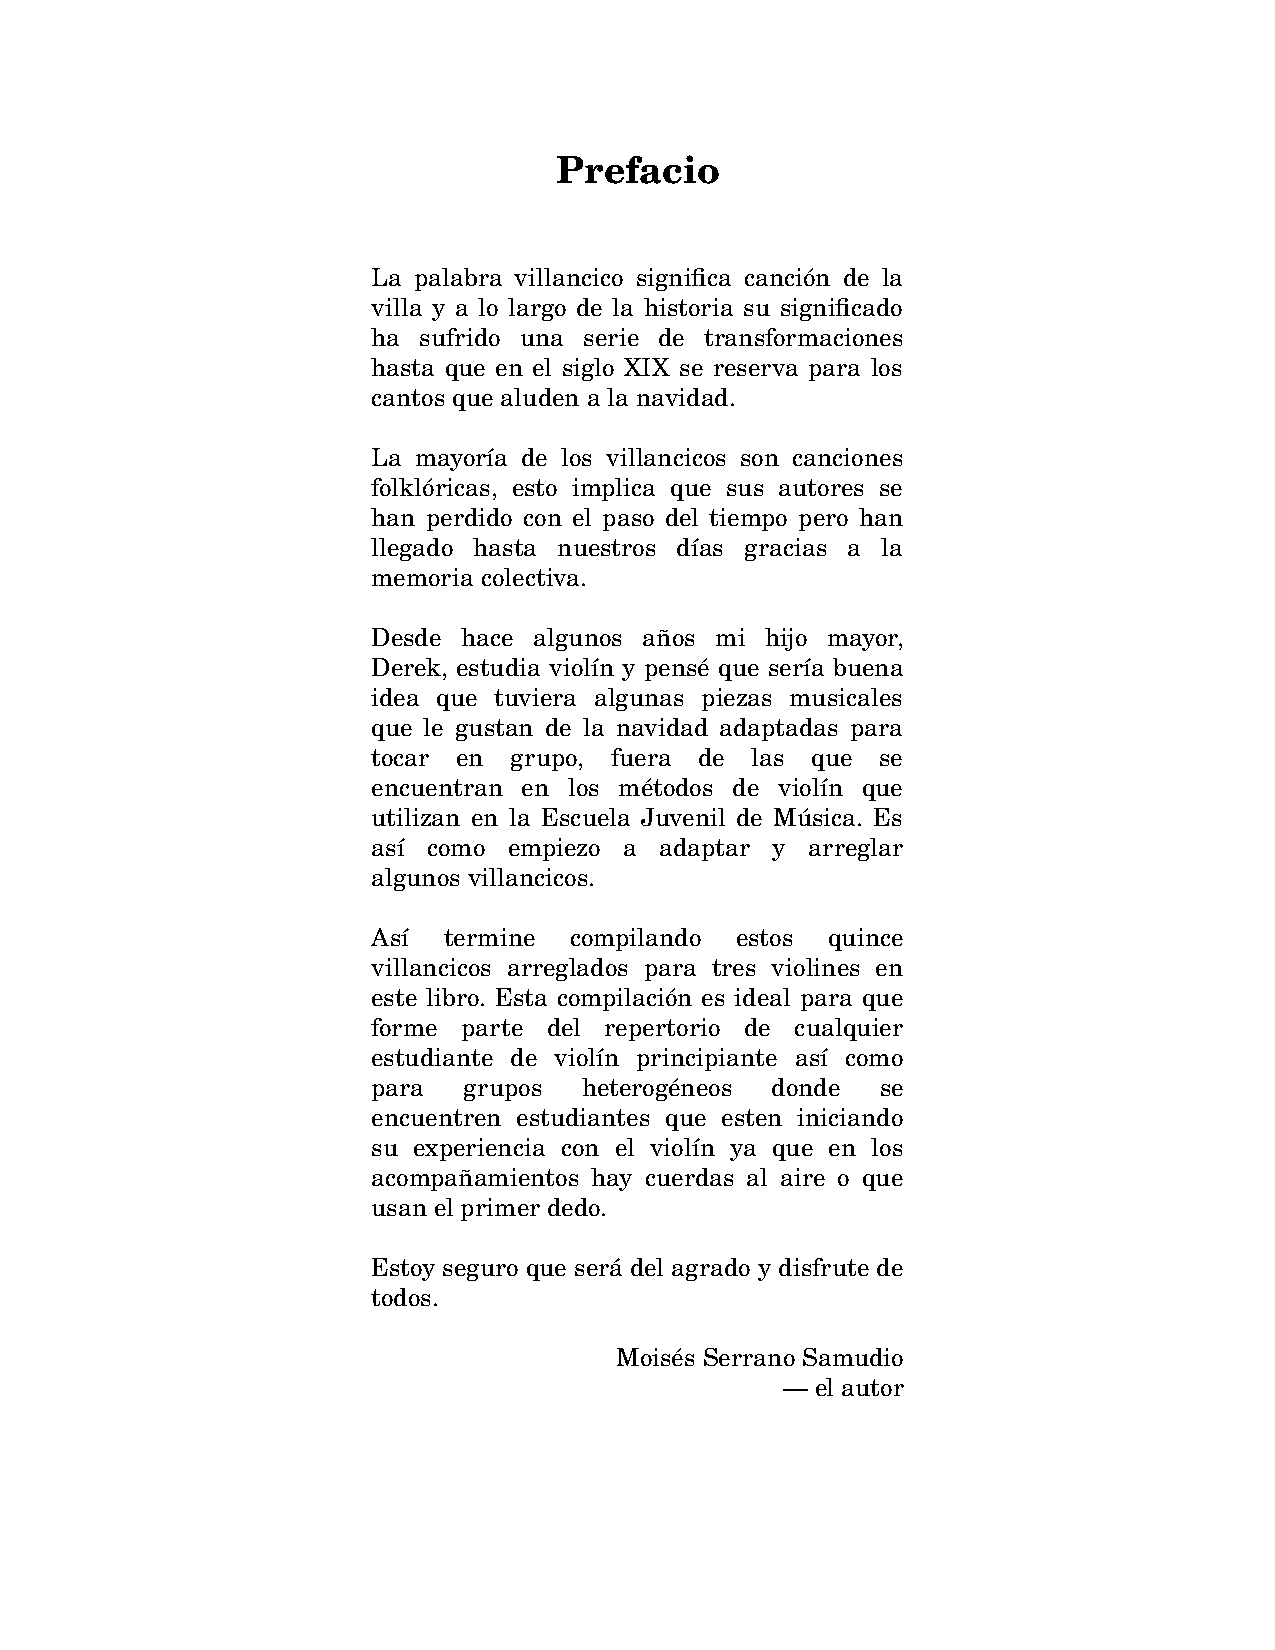
\includepdf[pages=-]{../extend/3-prefacio.pdf}
%\includepdf[pages=-]{../extend/6-chapter.pdf}
%
\includepdf[pages=-]{../extend/blank.pdf}

\pagenumbering{arabic}

\setcounter{secnumdepth}{-1} % elimina numeración de chapter para que no aparezca en toc

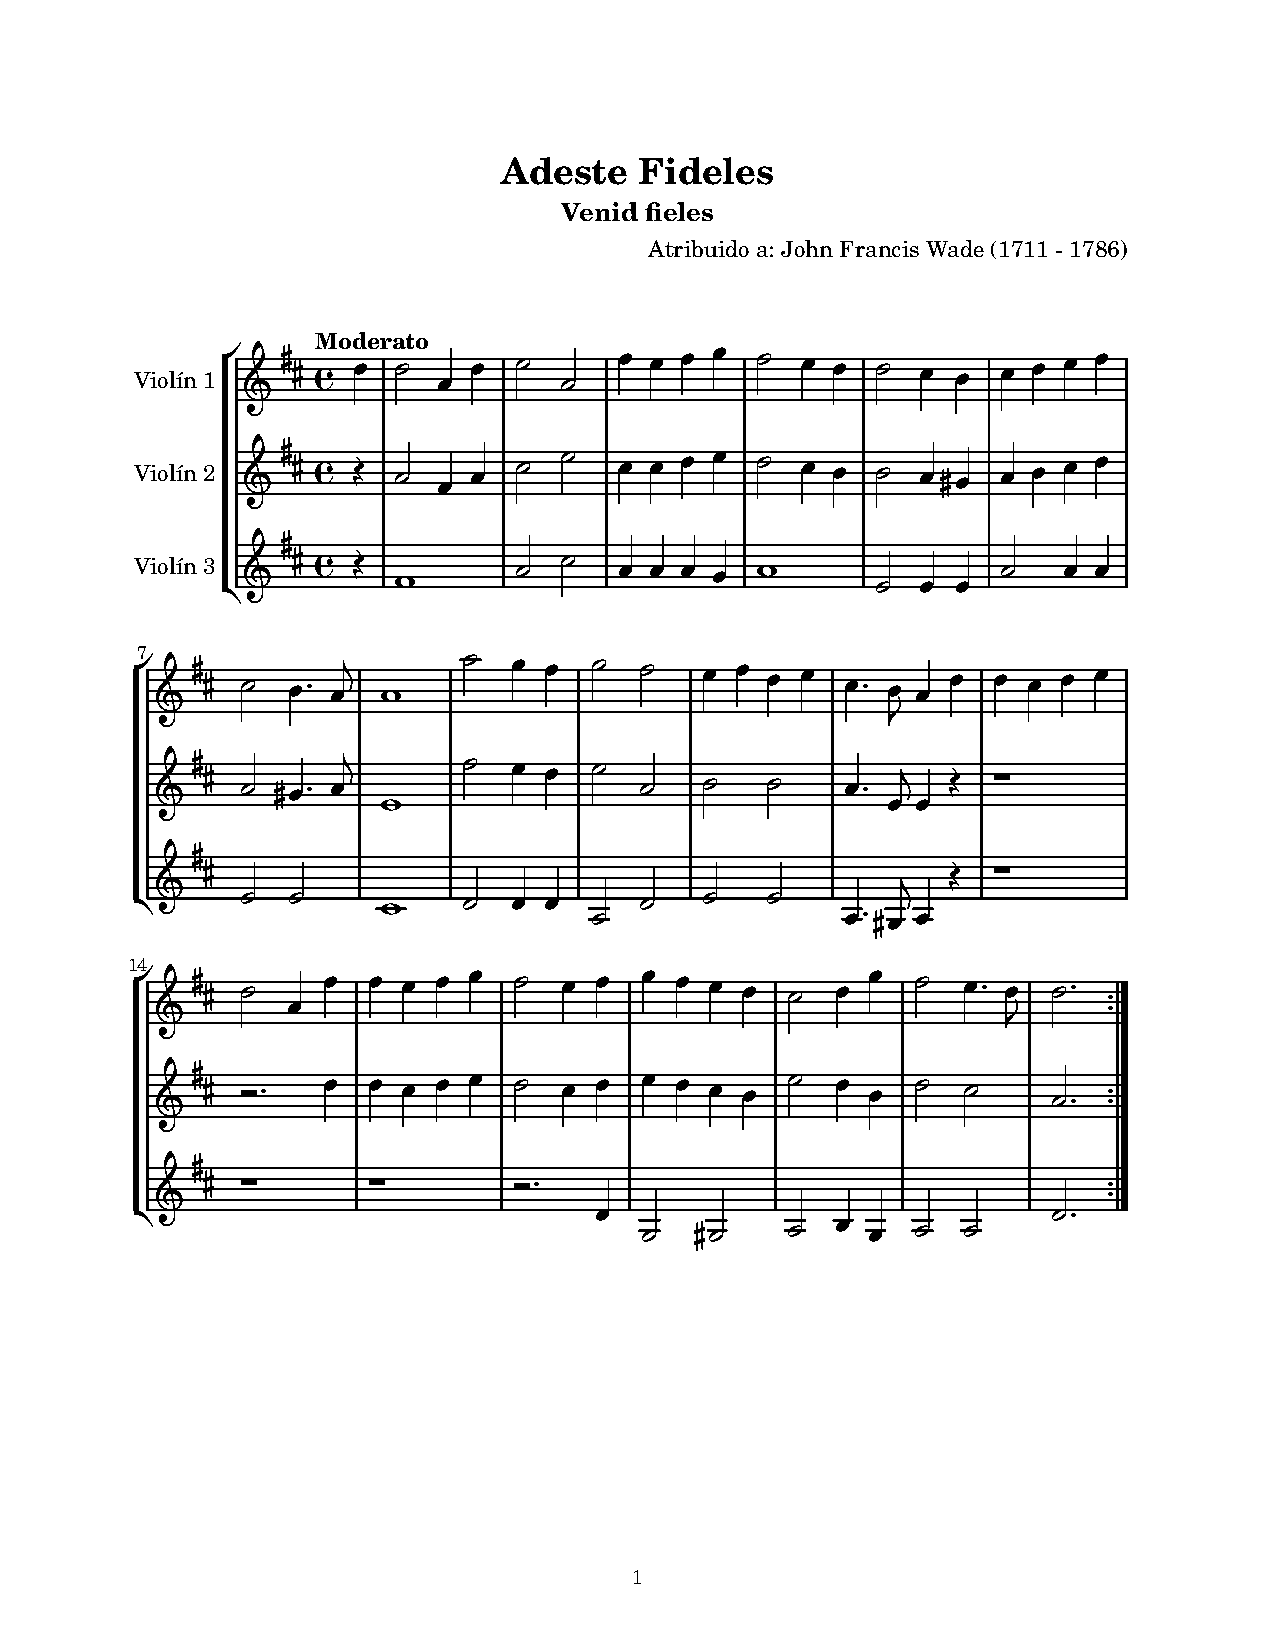
\includepdf[pages=-,addtotoc={
    1,chapter,1,Partituras,c1,
    1,section,2,Adeste Fideles,v1,
    2,section,2,Noche de Paz,v2,
    3,section,2,Campanas de Belén,v3, 
    4,section,2,Dime Niño,v4,
    6,section,2,{Fum, fum, fum},v5,
    8,section,2,Los peces en el río,v6,
    9,section,2,¡Ay del chiquirritin!,v7,
    10,section,2,La marimorena,v8,
    11,section,2,{Alegría, alegría},v9,
    12,section,2,{Rin, rin},v10,
    14,section,2,El niño del tambor,v11,
    16,section,2,Burrito sabanero,v12,
    18,section,2,Feliz Navidad,v13,
    19,section,2,Nochebuena panameña,v14,
    20,section,2,Arre borriquito,v15,
    23,section,2,{Extra: Nearer, My God, to Thee},extra,
    24,chapter,1,Letras,c2
    }]{../villancicos-compilados.pdf}


\includepdf[pages=-]{../extend/blank.pdf}

\renewcommand{\CoverName}{Colofón}%
\pagestyle{empty}%
\renewcommand{\thepage}{\CoverName}
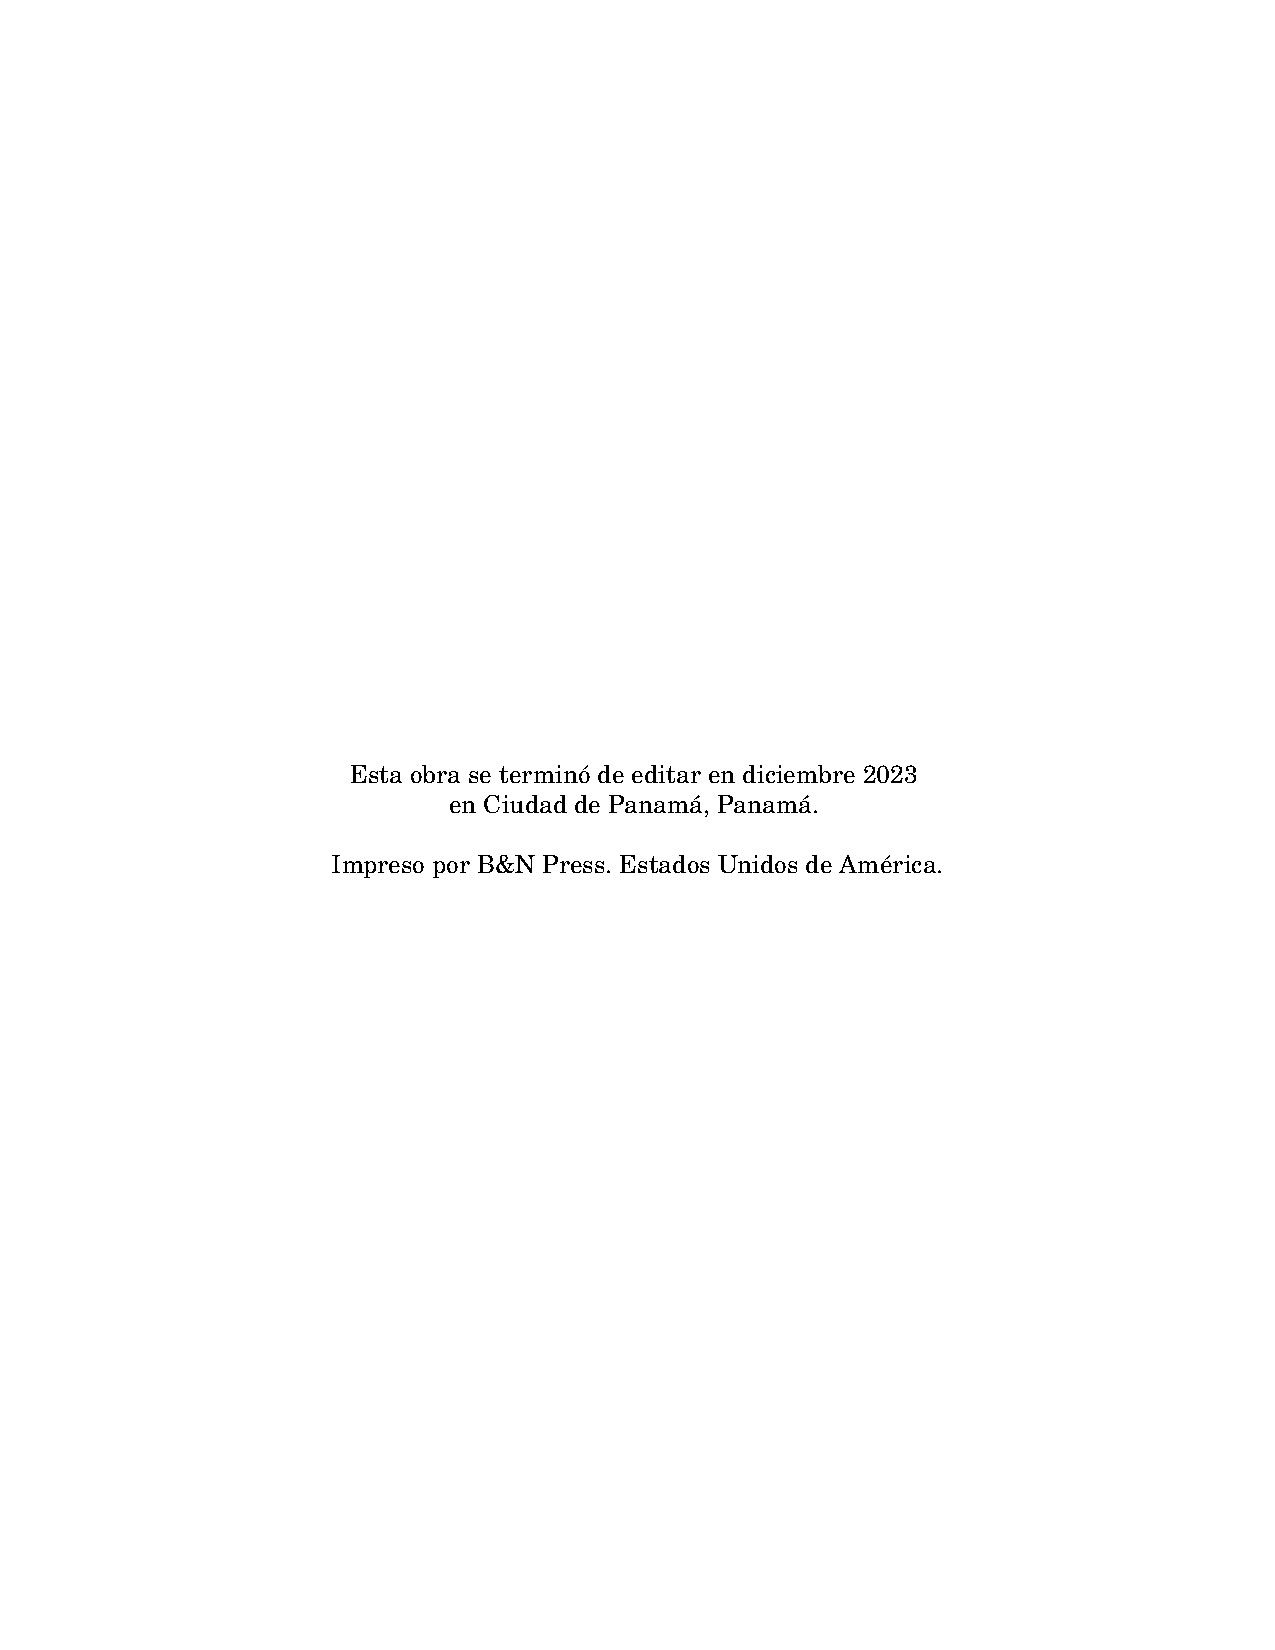
\includepdf[pages=-]{../extend/5-colofon.pdf}

\renewcommand{\CoverName}{Contraportada}%
\pagestyle{empty}%
\renewcommand{\thepage}{\CoverName}
\includepdf{../extend/contraportada.pdf}

\end{document}
